\documentclass{article}
    \usepackage{amssymb}
    \usepackage[utf8]{inputenc}
    \usepackage[russian]{babel}
    \usepackage[left=2cm,right=2cm,
        top=2cm,bottom=2cm,bindingoffset=0cm]{geometry}
    \usepackage{hyperref}
    \hypersetup{
        colorlinks=true,
        linkcolor=blue,
        filecolor=magenta,      
        urlcolor=cyan,
    }
  \usepackage{graphicx}
  \usepackage{booktabs}
  \graphicspath{{pictures/}}
  \DeclareGraphicsExtensions{.pdf,.png,.jpg}
\usepackage{subcaption}
%\captionsetup{compatibility=false}

\begin{document}
\begin{center}{\hugeОтчет по курсовой работе за неделю\\}\end{center}
Дата: 4.3.2021\\
Научные руководители: Герасимов С.В., Мещеряков А.В.\\
Студент: Немешаева Алиса\\
Курс: 4\\

\renewcommand{\labelitemi}{$\blacksquare$}
\renewcommand\labelitemii{$\square$}
\begin{enumerate}
    \item Изменены валидационная и тестовая области: теперь валидация - это западная часть неба, 
        а тест - восточная. Тренировочная выборка осталась без изменений. На таких данных была 
        обучена ещё одна модель all\_found4, все остальные её параметры повторяют модель all\_found.
        ~\ref{Fig:Val}\\
    \item Эта модель была обучена для получения графика recall по отношению к эпохе на восточной 
        тестовой выборке.~\ref{Fig:Recall}\\
    \item Изменены иллюстрации для демонстрации детектированных скоплений. Шаг сканирования 
        уменьшен до 4, добавлены координаты соседних скоплений.~\ref{Fig:Cluster}\\
\end{enumerate}




\begin{figure}[h]
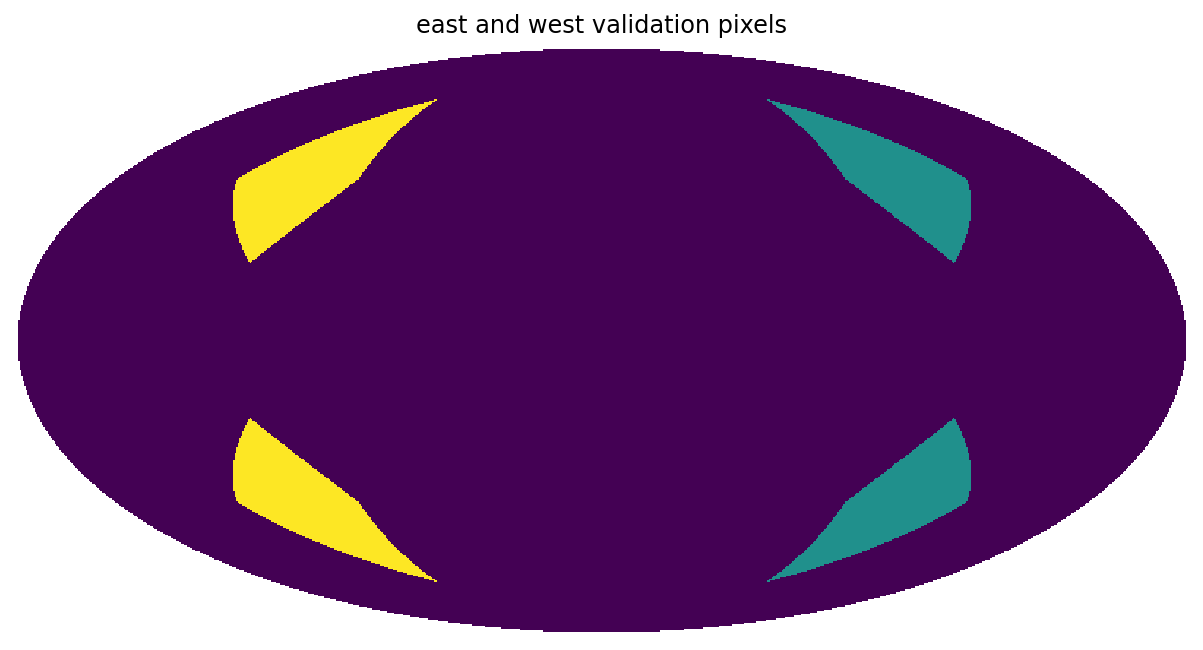
\includegraphics[width=0.6\linewidth]{val}
\caption{Распределение новых тестовой и валидационной областей.}
\label{Fig:Val}
\end{figure}

\begin{figure}[h]
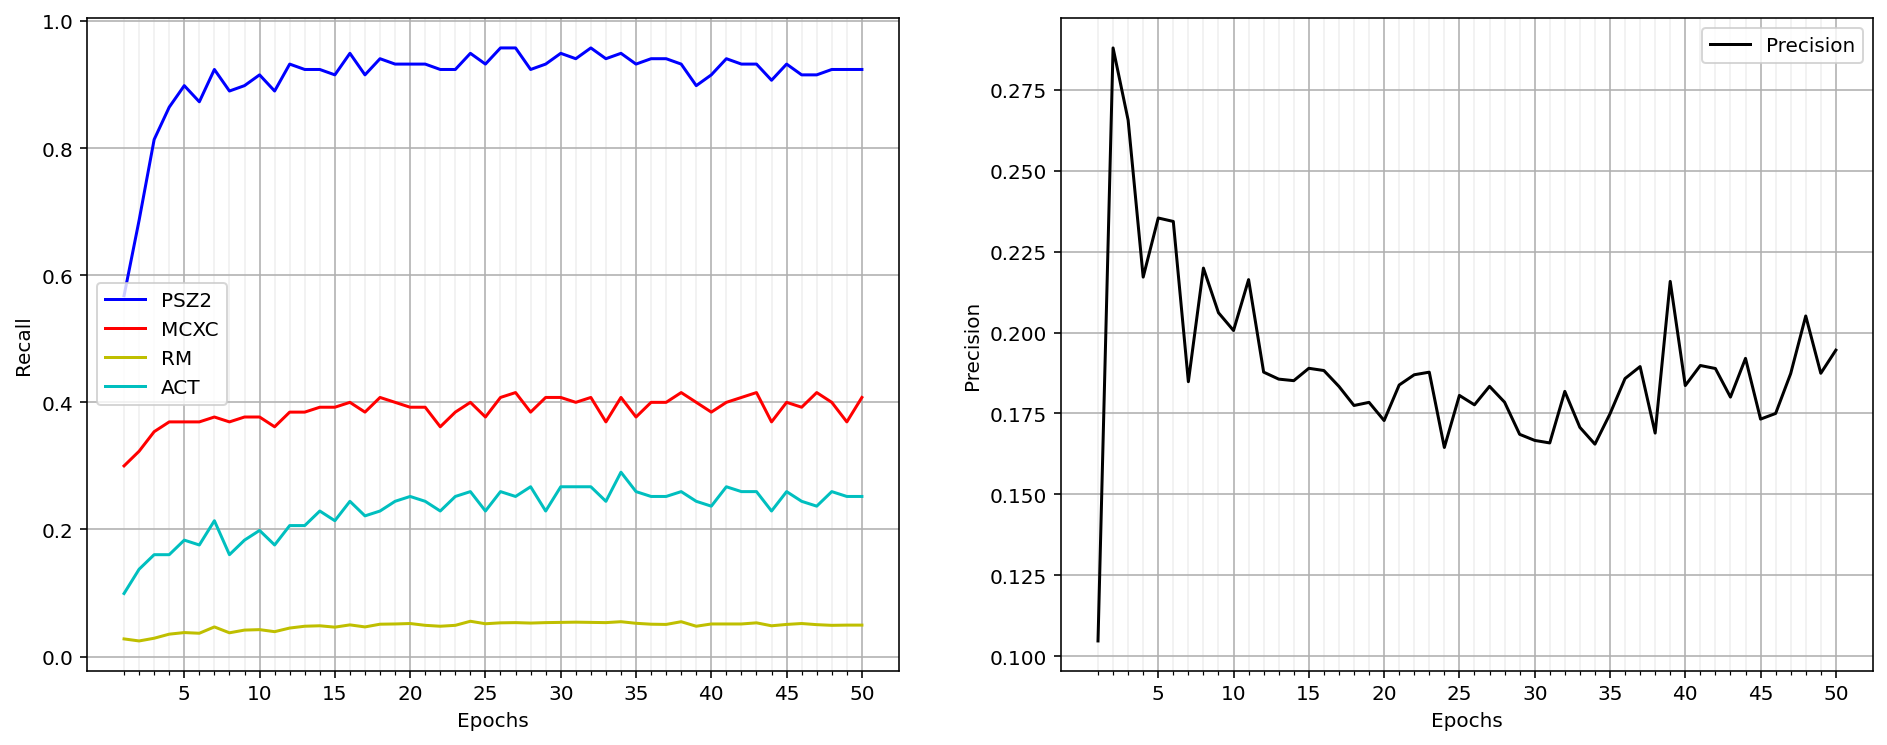
\includegraphics[width=0.8\linewidth]{recall}
\caption{Recall и precision для all\_found4.}
\label{Fig:Recall}
\end{figure}

\begin{figure}[h]
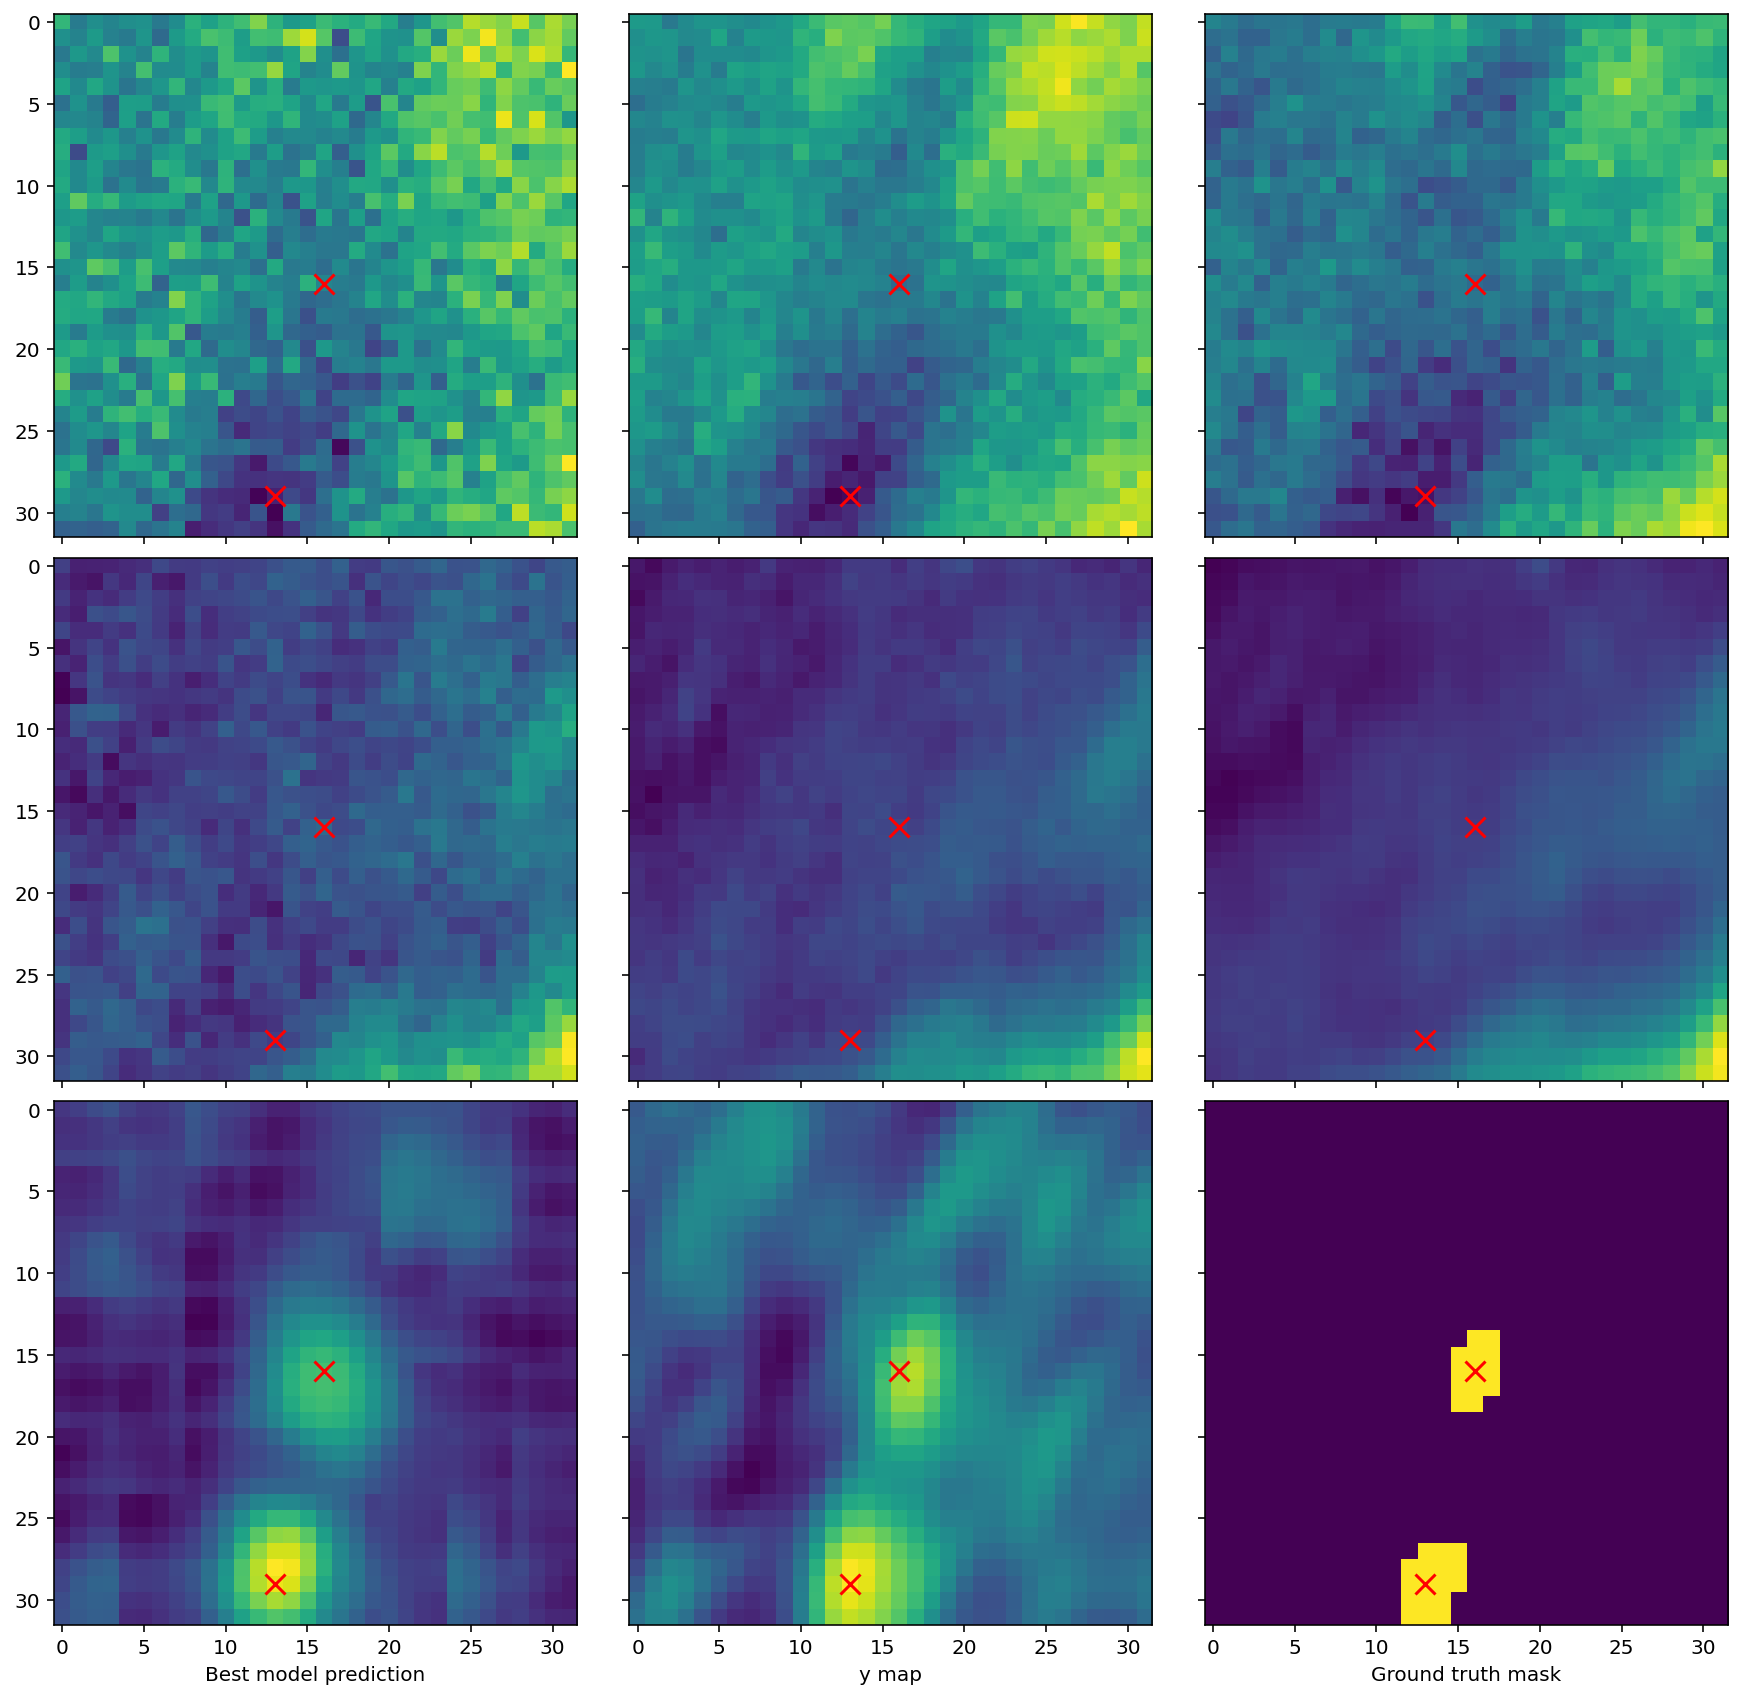
\includegraphics[width=0.6\linewidth]{cluster}
\caption{Новая версия иллюстрации для детектированного скопления (RA 2.55509, DEC 6.6322).}
\label{Fig:Cluster}
\end{figure}

Отчет согласован с научным руководителем.\\
Общее количество строк кода за эту неделю: 235\\
\href{https://github.com/rt2122/data-segmentation-2}{Репозиторий}\\ 
\end{document}
